\documentclass{sigchi}

% Use this command to override the default ACM copyright statement
% (e.g. for preprints).  Consult the conference website for the
% camera-ready copyright statement.


%% EXAMPLE BEGIN -- HOW TO OVERRIDE THE DEFAULT COPYRIGHT STRIP -- (July 22, 2013 - Paul Baumann)
\toappear{
{\emph{University of St Andrews}}, April 3, 2015, United Kingdom. \\
Copyright \copyright~Chi-Jui Wu. \\
}
%% EXAMPLE END -- HOW TO OVERRIDE THE DEFAULT COPYRIGHT STRIP -- (July 22, 2013 - Paul Baumann)


% Arabic page numbers for submission.  Remove this line to eliminate
% page numbers for the camera ready copy

%\pagenumbering{arabic}

% Load basic packages
\usepackage{balance}  % to better equalize the last page
\usepackage{graphics} % for EPS, load graphicx instead
%\usepackage[T1]{fontenc}
\usepackage{txfonts}
\usepackage{times}    % comment if you want LaTeX's default font
\usepackage[pdftex]{hyperref}
% \usepackage{url}      % llt: nicely formatted URLs
\usepackage{color}
\usepackage{textcomp}
\usepackage{booktabs}
\usepackage{ccicons}
\usepackage{todonotes}
\usepackage{svg}
\usepackage{amsmath}

% Set figures directory
\graphicspath{{./figures/}}
\setsvg{svgpath = figures/}

% llt: Define a global style for URLs, rather that the default one
\makeatletter
\def\url@leostyle{%
  \@ifundefined{selectfont}{\def\UrlFont{\sf}}{\def\UrlFont{\small\bf\ttfamily}}}
\makeatother
\urlstyle{leo}

% To make various LaTeX processors do the right thing with page size.
\def\pprw{8.5in}
\def\pprh{11in}
\special{papersize=\pprw,\pprh}
\setlength{\paperwidth}{\pprw}
\setlength{\paperheight}{\pprh}
\setlength{\pdfpagewidth}{\pprw}
\setlength{\pdfpageheight}{\pprh}

% Make sure hyperref comes last of your loaded packages, to give it a
% fighting chance of not being over-written, since its job is to
% redefine many LaTeX commands.
\definecolor{linkColor}{RGB}{6,125,233}
\hypersetup{%
  pdftitle={SIGCHI Conference Proceedings Format},
  pdfauthor={LaTeX},
  pdfkeywords={SIGCHI, proceedings, archival format},
  bookmarksnumbered,
  pdfstartview={FitH},
  colorlinks,
  citecolor=black,
  filecolor=black,
  linkcolor=black,
  urlcolor=linkColor,
  breaklinks=true,
}

% create a shortcut to typeset table headings
% \newcommand\tabhead[1]{\small\textbf{#1}}

% End of preamble. Here it comes the document.
\begin{document}

\title{Tracking People with Multiple Kinects}

\numberofauthors{1}
\author{%
  \alignauthor{Chi-Jui Wu\\
    \affaddr{Computer Science, University of St Andrews}\\
    \affaddr{United Kingdom}\\
    \email{cjw21@st-andrews.ac.uk}}\\
}

\maketitle

\begin{abstract}
This paper is my undergraduate thesis, completed in School of Computer Science, University of St Andrews, in 2015. The current work is a people tracking system consisted of multiple Kinects. The project aim is to track people in real world environments and resolve the occlusion problem. The final product contains an interactive software for tracking people and an user study on the developed system. The advantages and limitations of the system are discussed.
\end{abstract}

\keywords{Tracking; Occlusion; Kinect; Calibration; HCI}

\category{H.5.m.}{Information Interfaces and Presentation
  (e.g. HCI)}{Miscellaneous}{}{}

\section{Introduction}



\subsection{Problem statement}

The task of detecting and tracking moving targets in real world environment is non-trivial. There are many sources of tracking errors, such as sensor data noise and outliers, illumination levels, changing backgrounds, and occlusion. Real world environments are stochastic. Occlusion occurs when a tracked target is masked by other objects in existing fields of view. The position and movement of an occluded subject are unknown, hence increasing the difficulity of detection and tracking. Occlusions can be static and daynamic, as well as partial and full. Static occlusions refer to situations where stationary objects obstrct the visibility of the target, and dynamic occlusions occur during the interactions of many targets. Partial and full occlusion cases are when the target is partially and fully blocked from the view, respectively. THe current work attempts to resolve all different types of occlusion.

The problem is illustrated in Figure \ref{fig:occlusion_problem}.

\begin{figure}
  \centering
  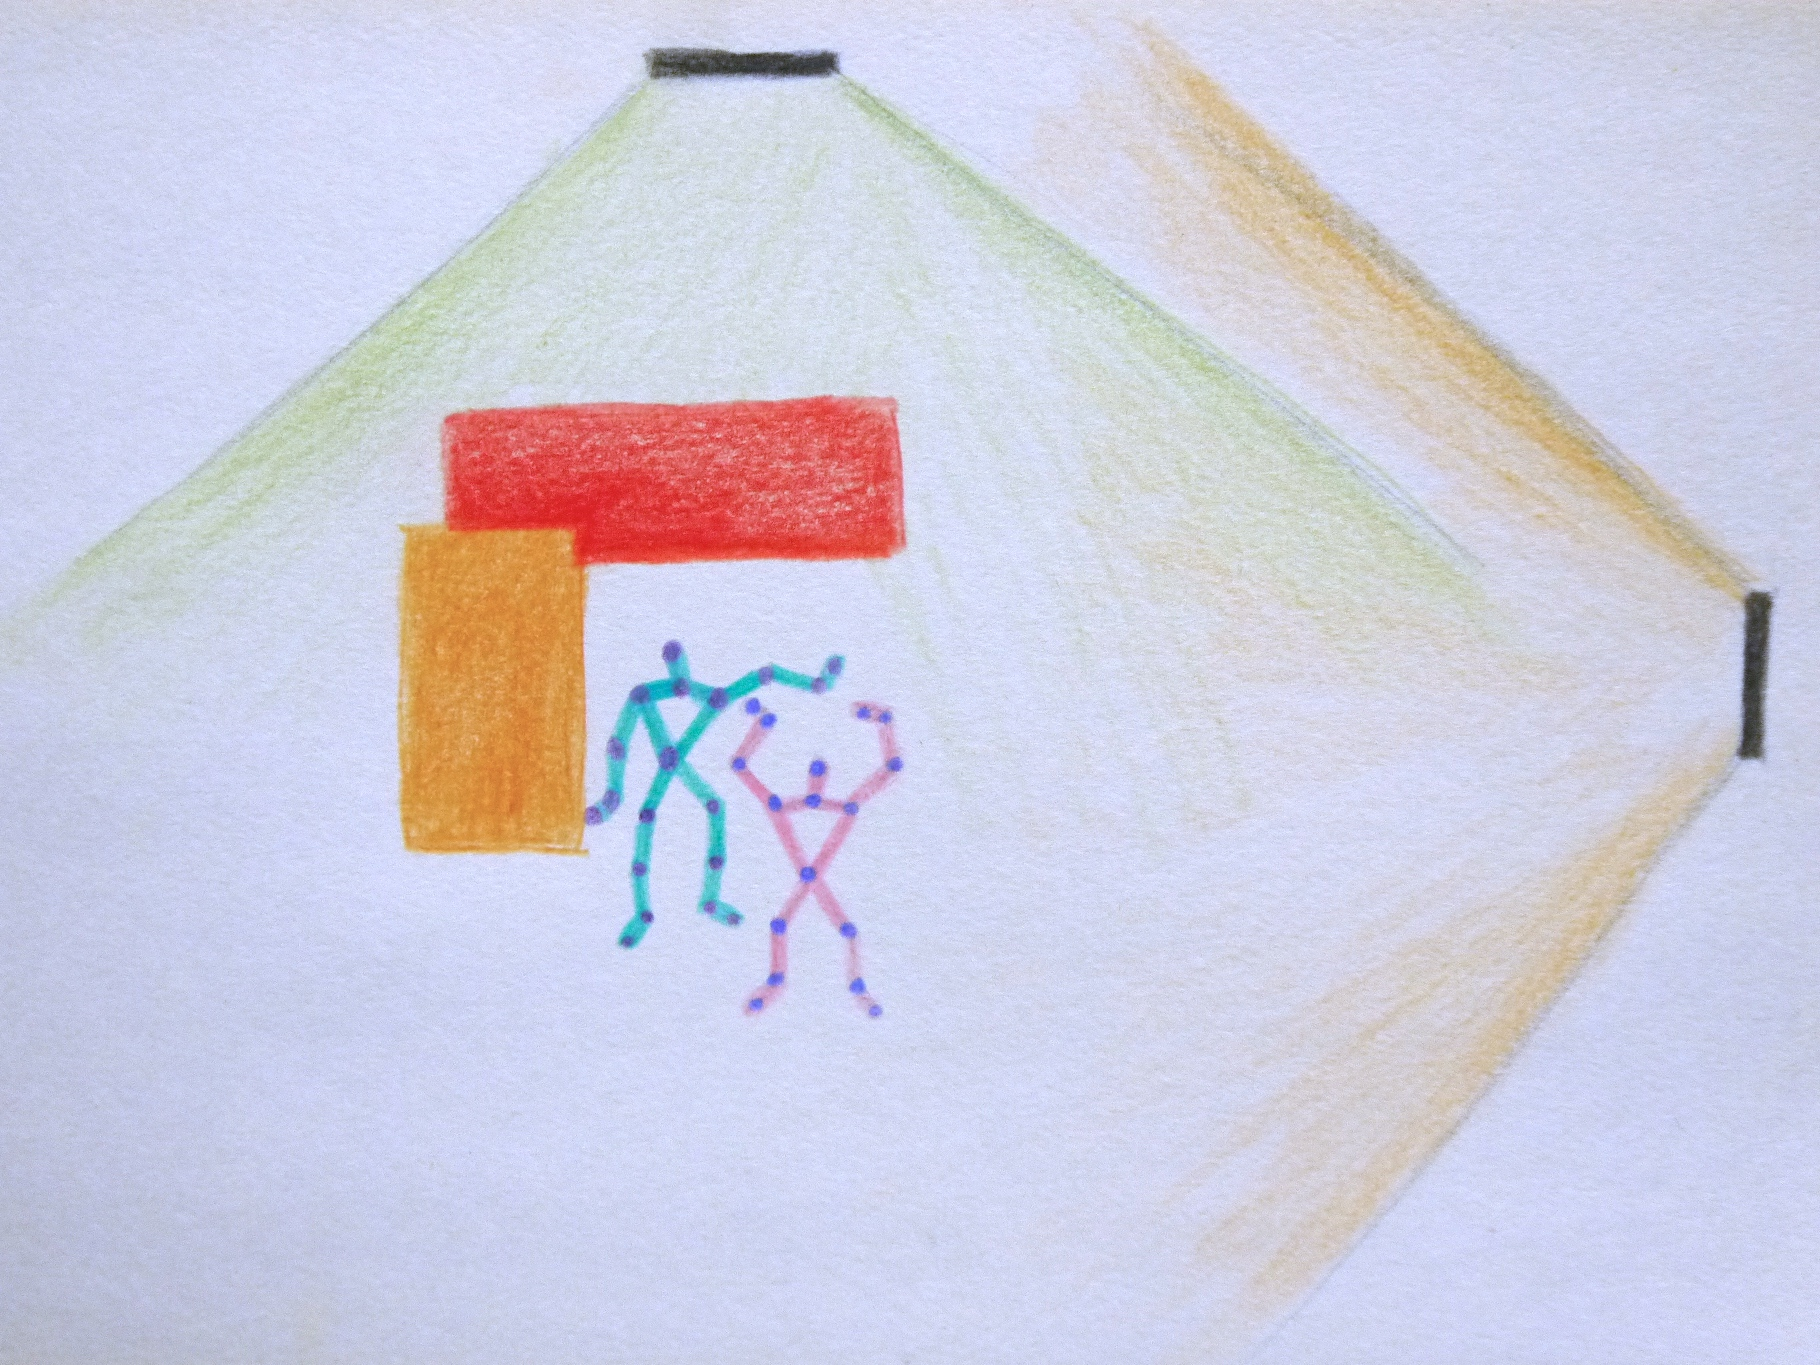
\includegraphics[width=0.9\columnwidth]{occlusion_problem}
  \caption{The occlusion problem}
  \label{fig:occlusion_problem}
\end{figure}

\subsection{Contributions}

Replicate current research, discuss limitations, (in)validate results. Resolve the problem of occlusion using multiple Kinects. 

\begin{enumerate}
  \item The first item
  \item The second item
  \item 
\end{enumerate}

\section{Previous Work}

Existing people detection and tracking techniques. Tracking people in surveillance video and in realtime. Tracking using mobile and wearable devices. Motion sensors and wireless. Time-of-flight and structured-light cameras.

[Paper: Particle filter to track multiple people for visual surveillance]
[Paper: Tracking People in Video Sequences by Clustering Feature Motion Paths]
[Paper: Evaluation of realtime people tracking for indoor environments using ubiquitous motion sensors and limited wireless network infrastructure]
[Paper: Tracking people under heavy occlusions by layered data association]
[Paper: Detection and Tracking of Occluded People]

\subsection{Tracking people}

\subsection{Coordiante transfomration}

\cite{wei_kinect_calibration}
\cite{eggert_four_algorithms}
\cite{horn_unit_quaternions}

\subsection{Tracking using depth data}

\subsection{Tracking using color data}

[Paper: Tracking people within groups using RGB-D data]
[Paper: Detecting and tracking people in real time with RGB-D camera]
[Paper: Applications for a people detection and tracking algorithm using a time-of-flight camera]
\*[Paper: Real-time Human Motion Tracking using Multiple Depth Cameras]
[Paper: Human Detection Using Depth Information by Kinect]

\section{Kinect}

The specification and components. Include image Larger field of views. Give examples.

\subsection{Features}

\subsection{Multiple Kinects}

\section{Current Approach}

\subsection{Overview}

The current system consists of two Kinects and two machines. Each machine is a client running one Kinect, and one machine 

\subsection{Computer Specification}

The server machine is running Microsoft Windows 8 on. The other client machine is running 

\subsection{Kinect Specification}

\subsection{Kinect Body Stream}

\subsection{Clients and Servers}

Clients sends the Kinect body stream to the server

\subsubsection{Communication Protocol}

\subsubsection{Serialization}

BodyFrame, Body, Joint. The important elements are the tracking state, joint type, amd camera space point.

\cite{microsoft_kinect_namespace}
\cite{microsoft_kinect_coordinates}

\subsection{Calibration}

\subsubsection{Technique}

Discuss the techniques from Wei et al.

\subsubsection{Detecting interference}

\subsection{Tracking by detection}

Skeletons from different Kinects matched based on spatial information. Filling the gaps of skeletons.

\subsection{Detecting occlusion}

\subsection{Detecting new skeletons}

\subsection{Strength}

\subsection{Limitations}

\subsection{Improvements}

\section{Testing}

Interactive application. View the average and individual skeletons from different Kinect fields of views.

\begin{figure}
  \centering
  
\includegraphics[width=0.9\columnwidth]{ui}
  \caption{UI}
  \label{fig:ui}
\end{figure}

\subsection{Occlusion}

Show persistent tracking in occluded environments. Demonstrate the system works with complex human interactions.
 
\section{Evaluation}

Discuss results. Compre them with Wei et al.

\subsection{User studies}

\begin{figure}
  \centering
  \includesvg[width=0.9\columnwidth]{stationary_p0_d7_all}
  \caption{One person all joints}~\label{fig:one_person_all}
\end{figure}

\begin{figure}
  \centering
  \includesvg[width=0.9\columnwidth]{stationary_p0_d7_average}
  \caption{One person average}~\label{fig:one_person_average}
\end{figure}

\begin{figure}
  \centering
  \includesvg[width=0.9\columnwidth]{scenarios}
  \caption{All scenarios}~\label{fig:scenarios}
\end{figure}

\subsection{Study 1}

\subsection{Study 2}

\subsection{Study 3}

\subsection{Study 4}

\subsection{Study 5}

\subsection{Study 6}

\subsection{Occlusion}

User study with multiple people and obstacles.

\section{Application}

Features

\subsection{Tracking UI}

\subsection{Disjoined UI}

\textbf{``Disjoined'' or called something else}

\subsection{Integration with Heart Rate Monitoring}

\section{Future Work}

\subsection{User studies}

\subsection{Application}

\section{SH Project Reflection}

SECTION

\subsection{Requirements Specification}

\section{Acknowledgments}

SECTION

% Balancing columns in a ref list is a bit of a pain because you
% either use a hack like flushend or balance, or manually insert
% a column break.  http://www.tex.ac.uk/cgi-bin/texfaq2html?label=balance
% multicols doesn't work because we're already in two-column mode,
% and flushend isn't awesome, so I choose balance.  See this
% for more info: http://cs.brown.edu/system/software/latex/doc/balance.pdf
%
% Note that in a perfect world balance wants to be in the first
% column of the last page.
%
% If balance doesn't work for you, you can remove that and
% hard-code a column break into the bbl file right before you
% submit:
%
% http://stackoverflow.com/questions/2149854/how-to-manually-equalize-columns-
% in-an-ieee-paper-if-using-bibtex
%
% Or, just remove \balance and give up on balancing the last page.
%
\balance{}

% REFERENCES FORMAT
% References must be the same font size as other body text.
\bibliographystyle{SIGCHI-Reference-Format}
\bibliography{report_bib}

\end{document}

%%% Local Variables:
%%% mode: latex
%%% TeX-master: t
%%% End:
